%% LyX 2.1.1 created this file.  For more info, see http://www.lyx.org/.
%% Do not edit unless you really know what you are doing.
\documentclass[english]{beamer}
\usepackage[T1]{fontenc}
\usepackage[latin9]{inputenc}
\setcounter{secnumdepth}{3}
\setcounter{tocdepth}{3}
\usepackage{array}
\usepackage{bm}
\usepackage{multirow}
\usepackage{amsmath}
\usepackage{graphicx}
\usepackage{esint}

\makeatletter

%%%%%%%%%%%%%%%%%%%%%%%%%%%%%% LyX specific LaTeX commands.
%% Because html converters don't know tabularnewline
\providecommand{\tabularnewline}{\\}

%%%%%%%%%%%%%%%%%%%%%%%%%%%%%% Textclass specific LaTeX commands.
 % this default might be overridden by plain title style
 \newcommand\makebeamertitle{\frame{\maketitle}}%
 % (ERT) argument for the TOC
 \AtBeginDocument{%
   \let\origtableofcontents=\tableofcontents
   \def\tableofcontents{\@ifnextchar[{\origtableofcontents}{\gobbletableofcontents}}
   \def\gobbletableofcontents#1{\origtableofcontents}
 }

%%%%%%%%%%%%%%%%%%%%%%%%%%%%%% User specified LaTeX commands.
%\usetheme{Warsaw}
\usetheme{amcg}
%\usepackage{eulervm}
\usepackage{bm}
% or ...

%\usecolortheme{orchid}
%\setbeamertemplate{footline}[text line]{} % makes the footer EMPTY

\setbeamercovered{transparent}
% or whatever (possibly just delete it)

\makeatother

\usepackage{babel}
\begin{document}





\title[Mesh Adaptivity and Fluidity]{Mesh Adaptivity and Fluidity}


\author[James Percival]{James~Percival}


\institute[AMCG]{AMCG,\\
Department of Earth Science and Engineering\\
Imperial College London}


\date[Fluidity Training 2014]{Fluidity Training 2014}

\makebeamertitle


%\pgfdeclareimage[height=0.5cm]{institution-logo}{institution-logo-filename}

%\logo{\pgfuseimage{institution-logo}}



%\AtBeginSubsection[]{
%  \frame<beamer>{ 
%    \frametitle{Outline}   
%    \tableofcontents[currentsection,currentsubsection] 
%  }
%}



%\beamerdefaultoverlayspecification{<+->}
\begin{frame}{Outline}


\tableofcontents{}

\end{frame}

\section{Mesh Adaptivity}


\subsection{Grids and meshes in computational science}
\begin{frame}{Grids \& Meshes}




Aside from spectral/particle based methods, computational grids and
meshes are ubiquitous in computational science:
\begin{itemize}
\item \emph{Grids} of \emph{points} for finite difference methods
\item Tesselations of subvolumes for finite volume methods
\item Tesselations of elements for finite element methods
\end{itemize}

\begin{center}
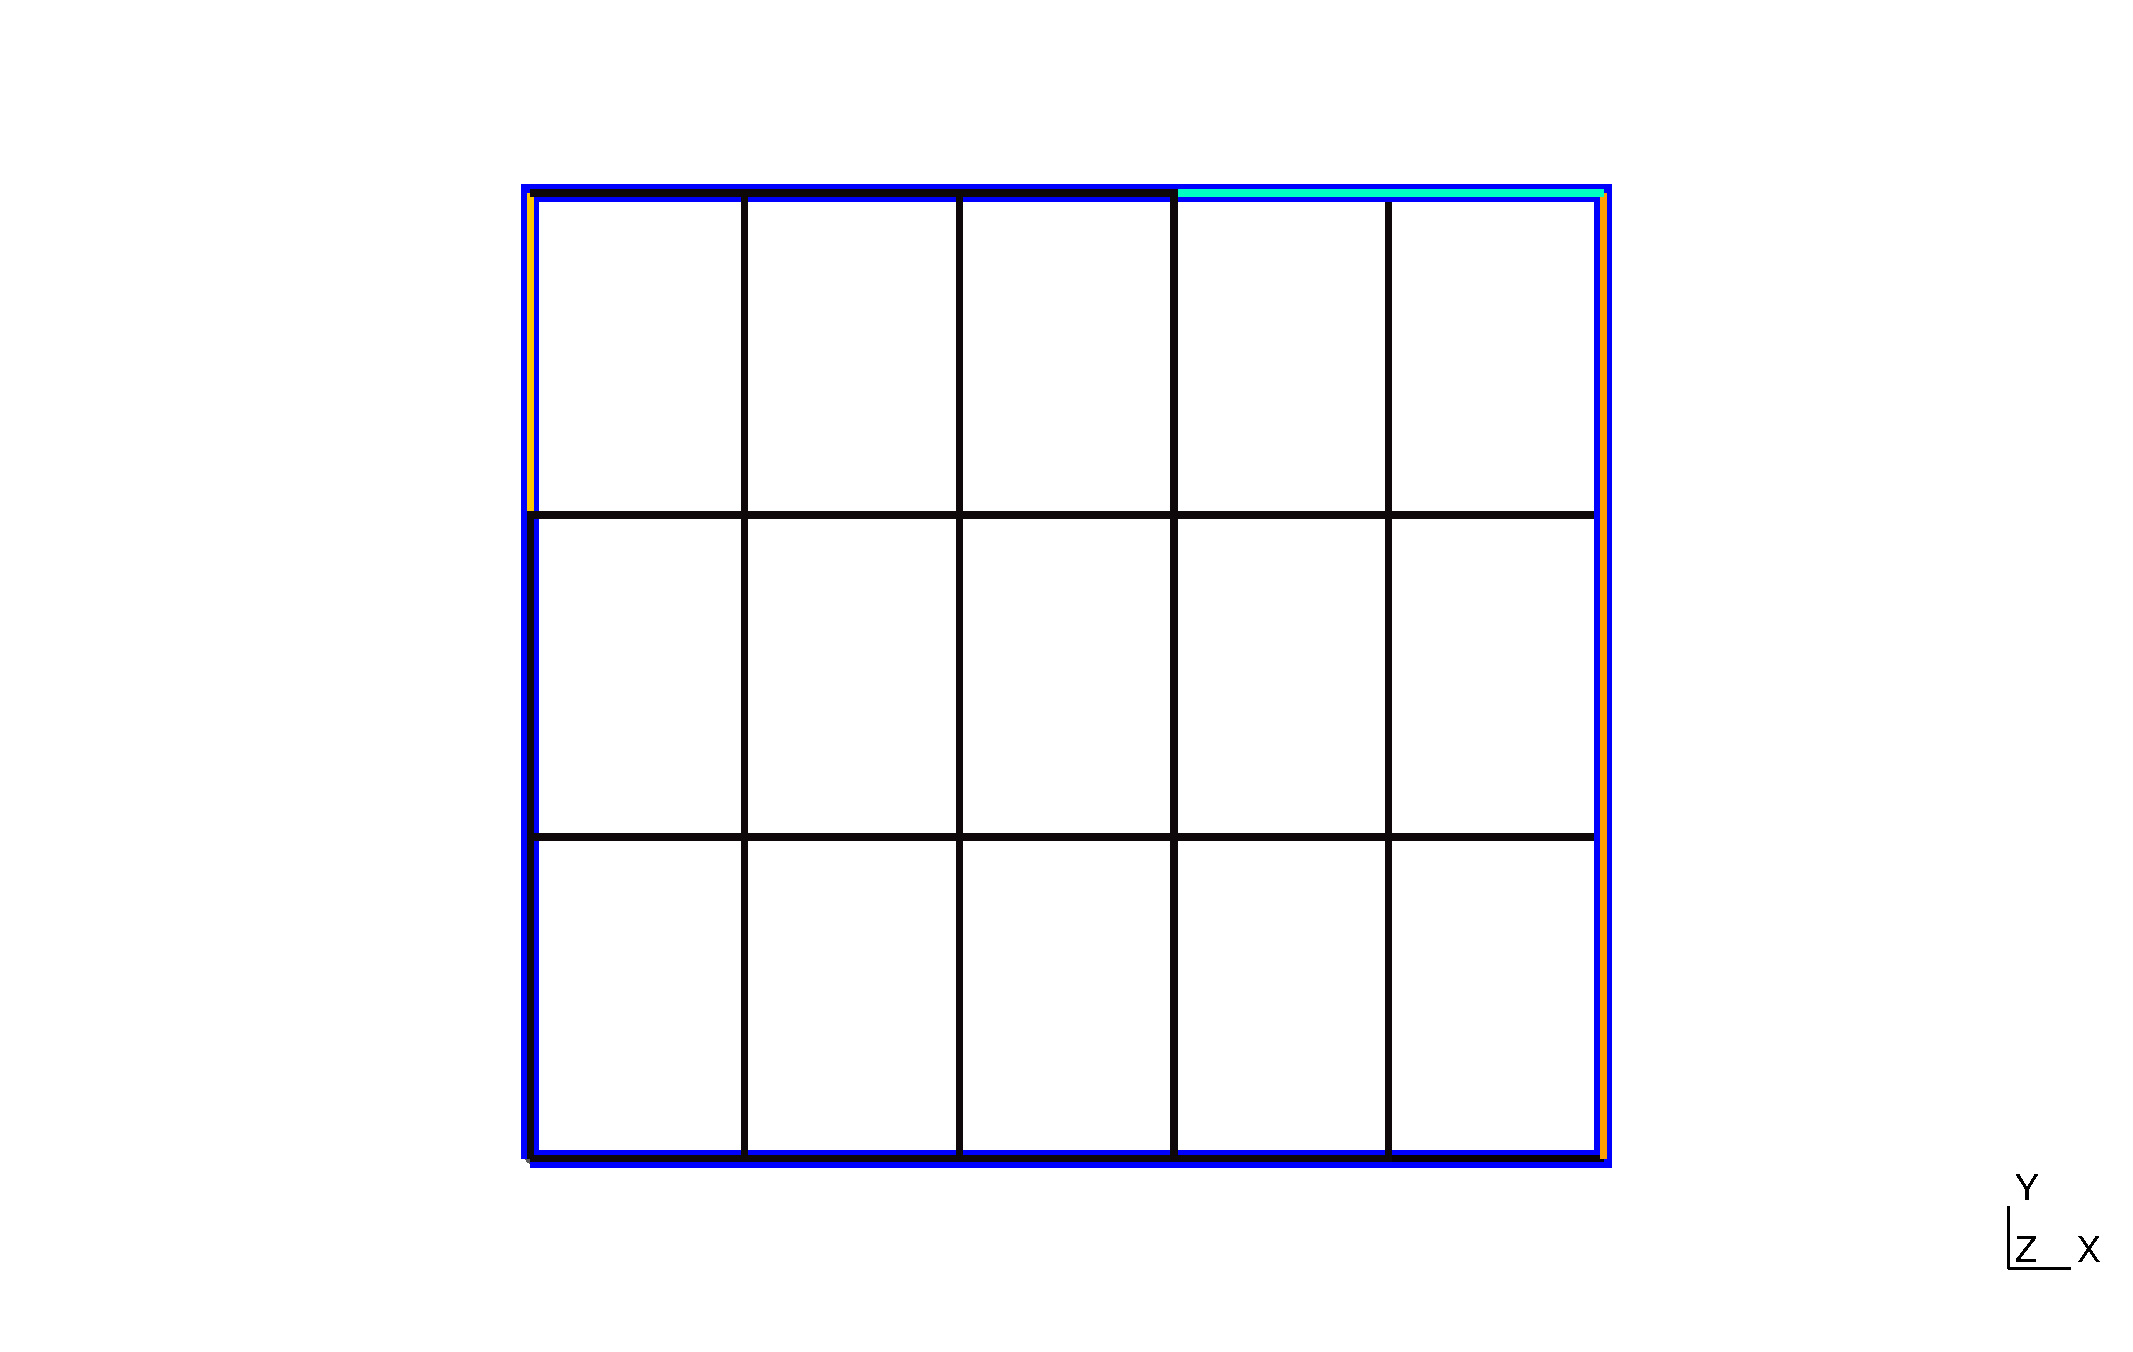
\includegraphics[width=0.25\textwidth]{Uniform}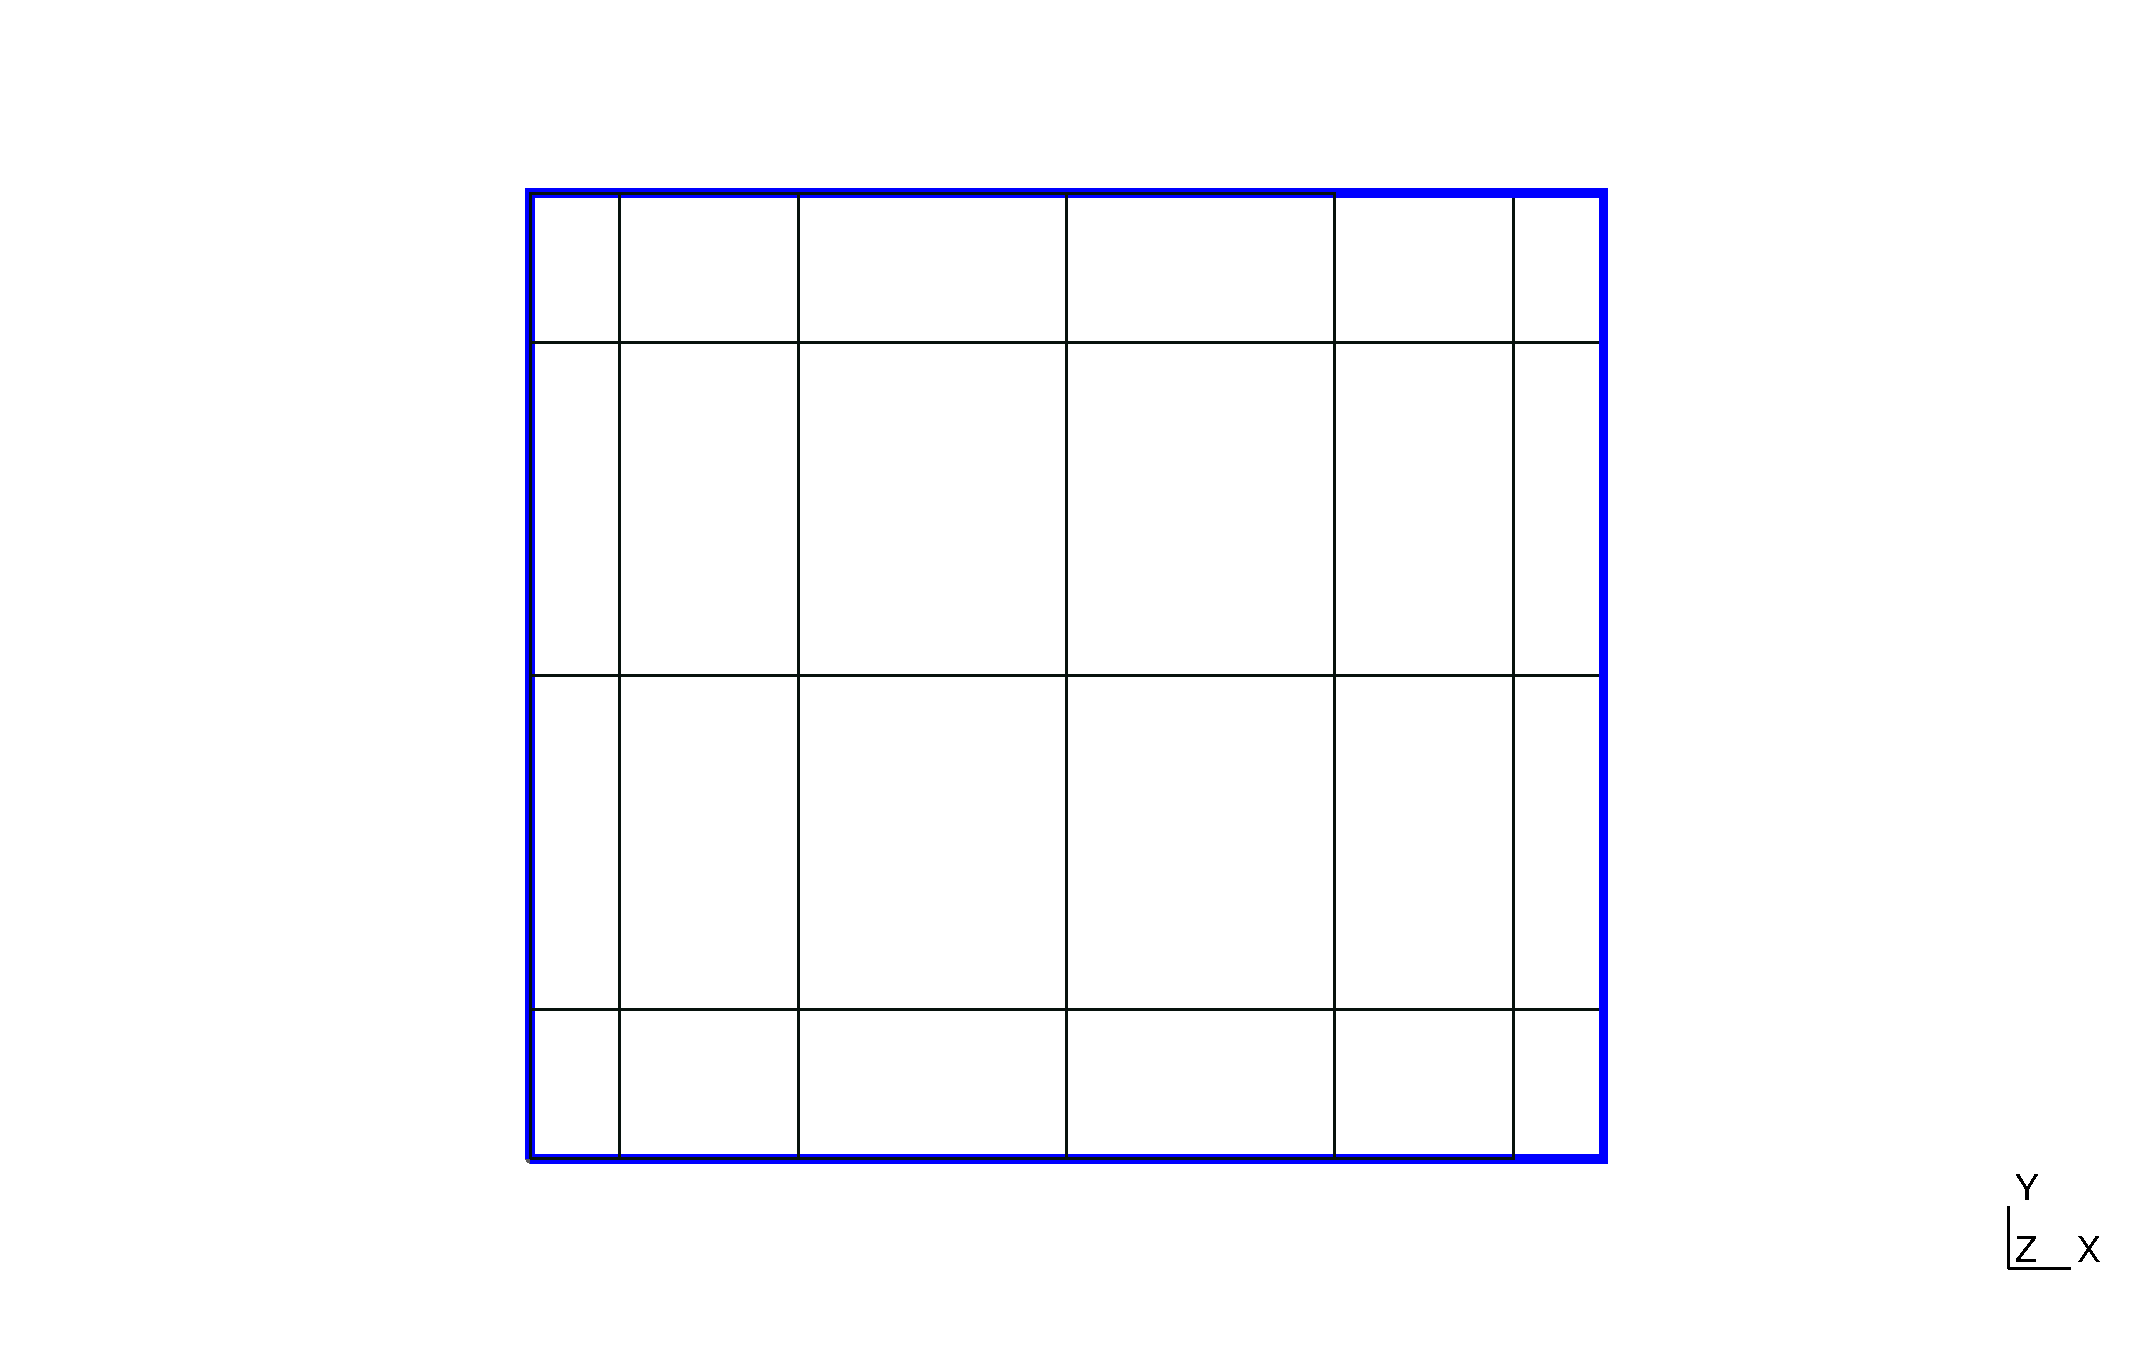
\includegraphics[width=0.25\textwidth]{Nonuniform}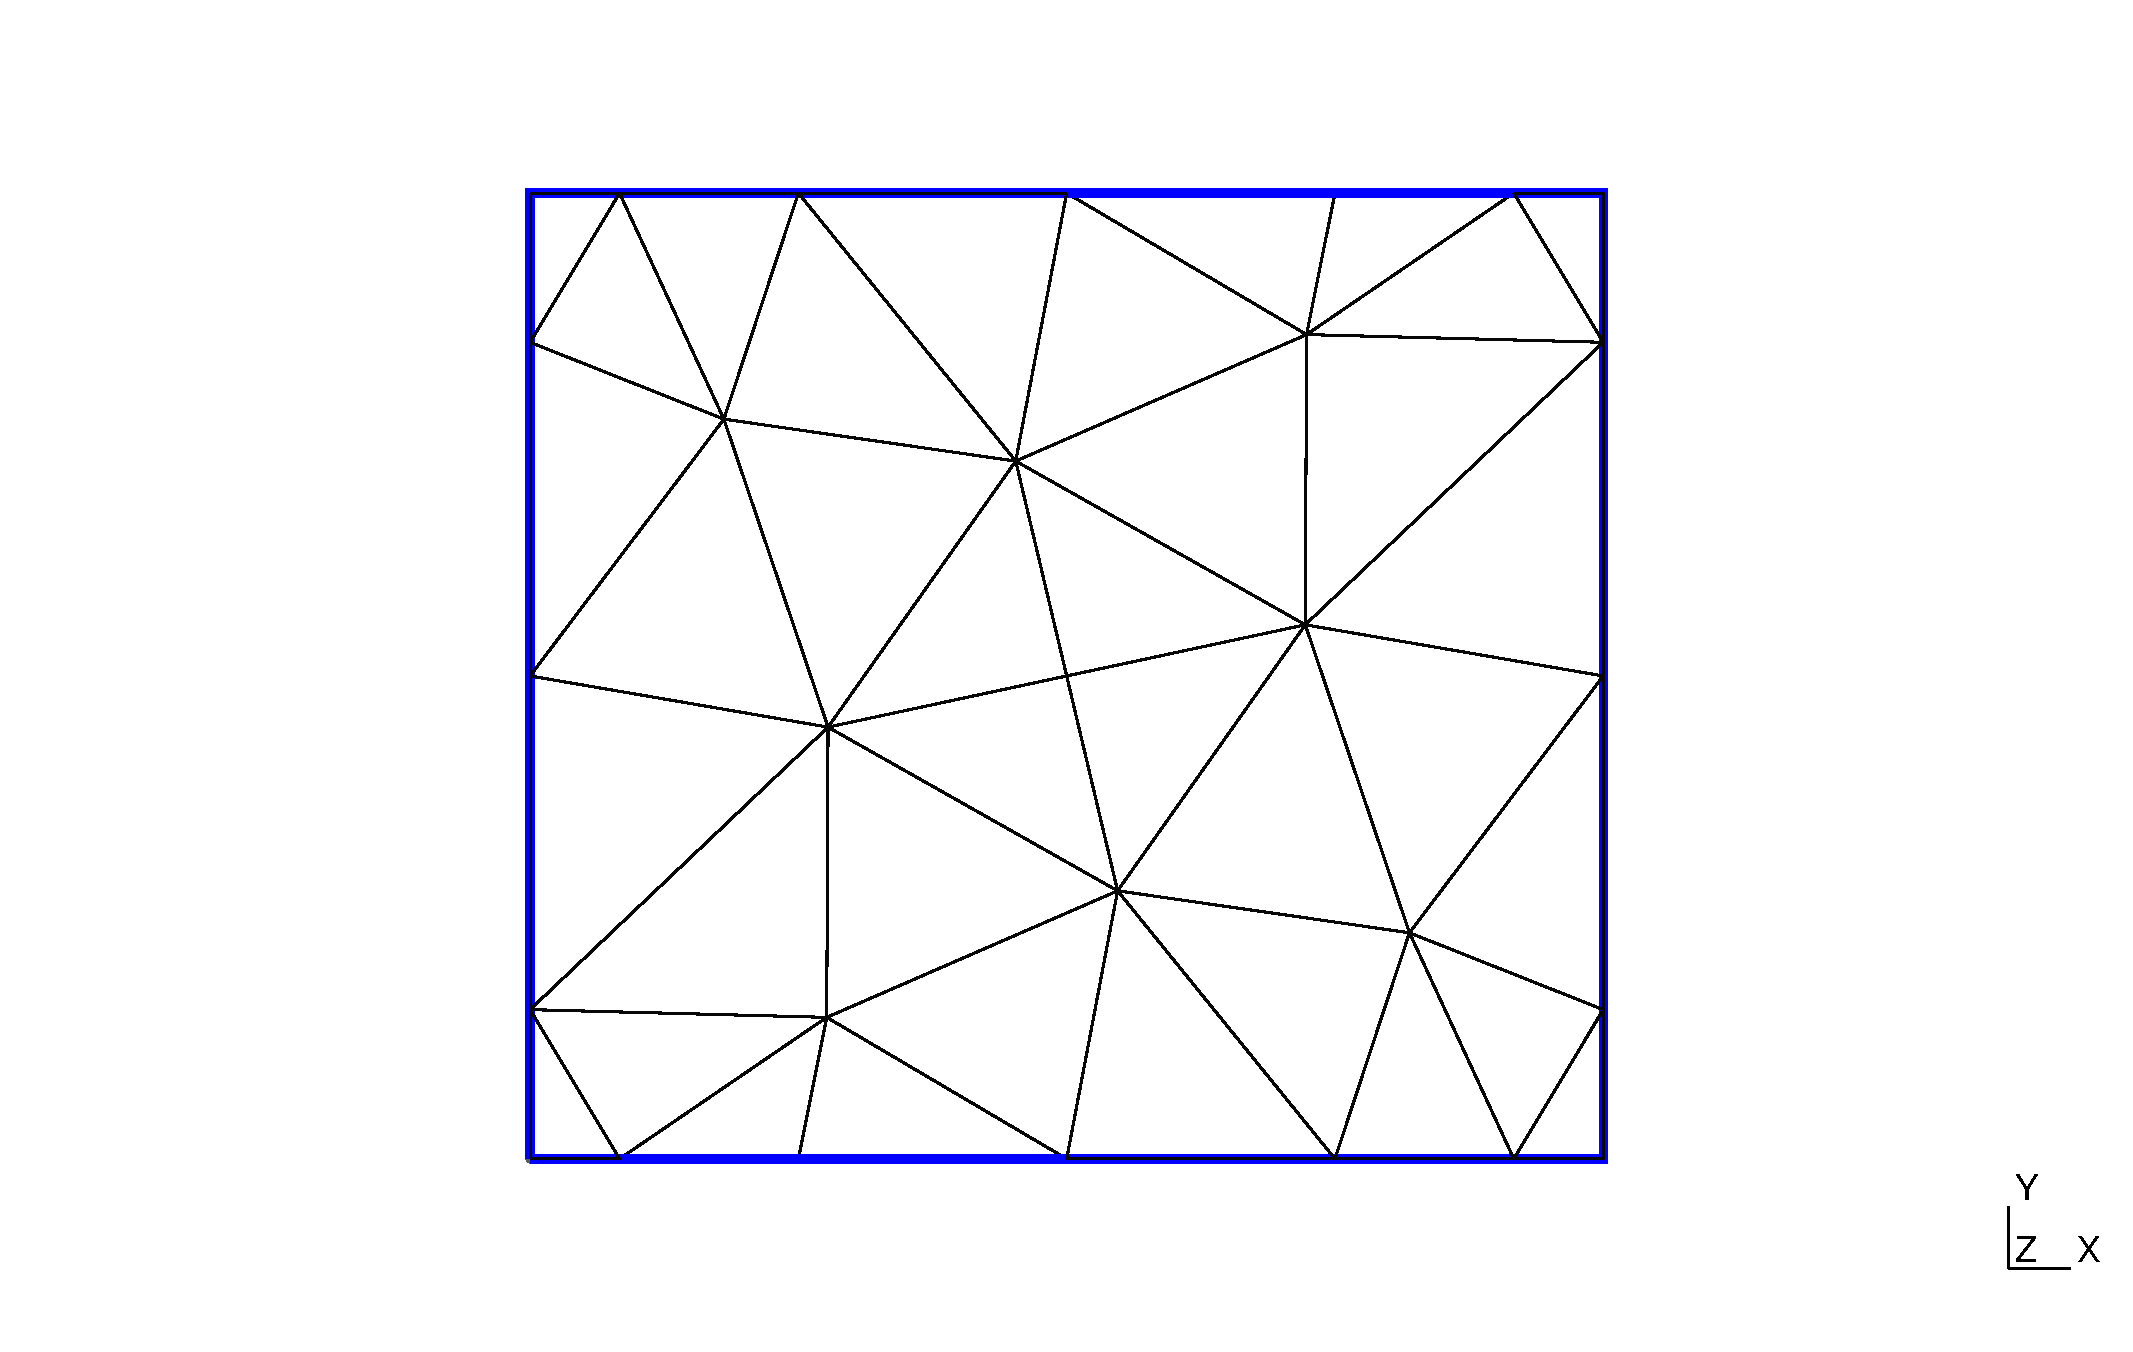
\includegraphics[width=0.25\textwidth]{Unstructured}
\par\end{center}

\end{frame}

\begin{frame}{Grids \& Meshes}




Meshes/grids:
\begin{itemize}
\item can be structured or \emph{unstructured}.
\item describe \emph{geometry} of problem.
\item define a local resolvable \emph{resolution}.
\item help determine bounds on solution error.
\end{itemize}

Frequently fine resolution is only required in limited regions, which
change with time.


Idea: progressively modify the mesh to put resolution where it is
needed.

\end{frame}



\subsection{Adaptive Mesh Refinement}
\begin{frame}{Adaptive Mesh Refinement (AMR)}


When this idea is followed through on structured meshes, it is often
called adaptive mesh refinement. Blocks are subdivided in areas of
refinement. Good for computer memory access, less good for physics.


\vspace{-2.65cm}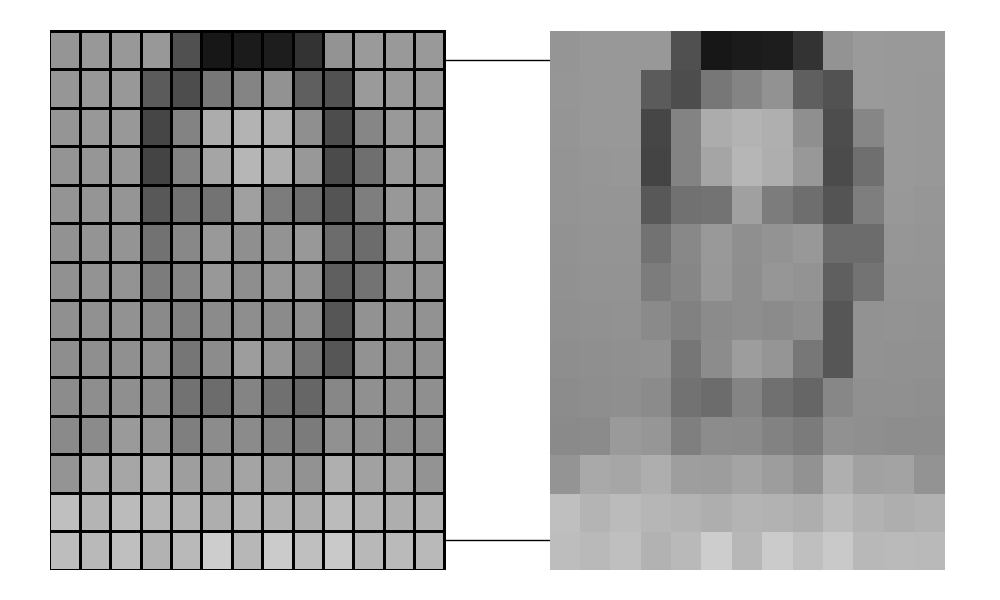
\includegraphics[bb=0bp 0bp 1000bp 600bp,clip,scale=0.45]{MDP_00}

\end{frame}

\begin{frame}{Adaptive Mesh Refinement (AMR)}


When this idea is followed through on structured meshes, it is often
called adaptive mesh refinement. Blocks are subdivided in areas of
refinement. Good for computer memory access, less good for physics.


\vspace{-2.65cm}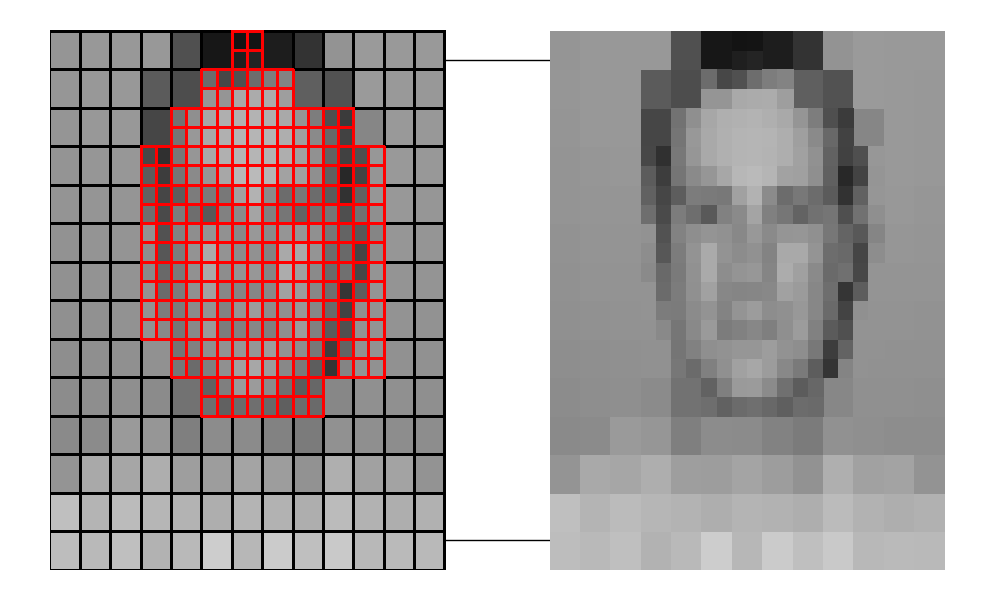
\includegraphics[bb=0bp 0bp 1000bp 600bp,clip,scale=0.45]{MDP_01}

\end{frame}

\begin{frame}{Adaptive Mesh Refinement (AMR)}


When this idea is followed through on structured meshes, it is often
called adaptive mesh refinement. Blocks are subdivided in areas of
refinement. Good for computer memory access, less good for physics.


\vspace{-2.65cm}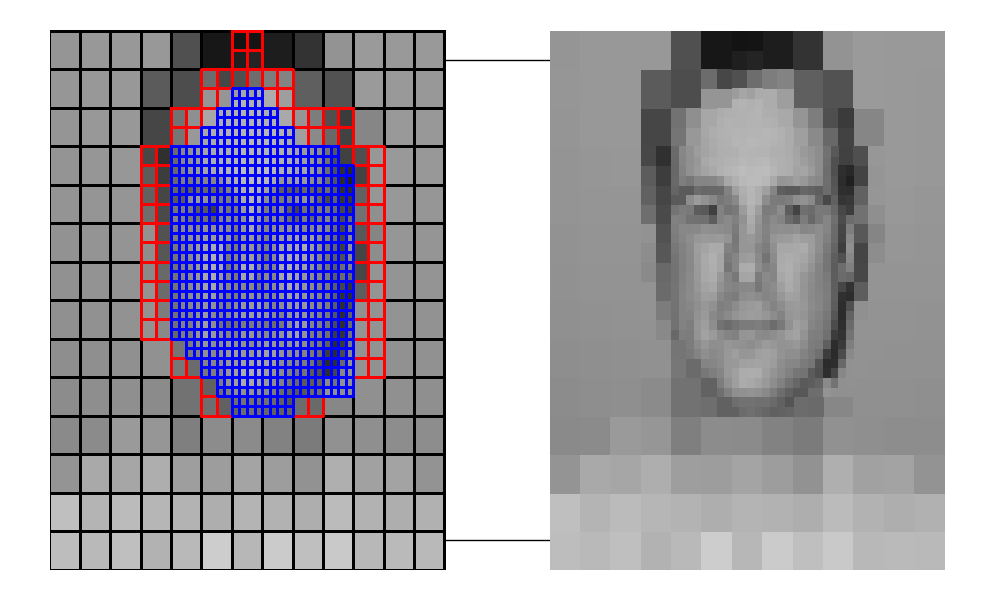
\includegraphics[bb=0bp 0bp 1000bp 600bp,clip,scale=0.45]{MDP_02}

\end{frame}

\begin{frame}{Adaptive Mesh Refinement (AMR)}


When this idea is followed through on structured meshes, it is often
called adaptive mesh refinement. Blocks are subdivided in areas of
refinement. Good for computer memory access, less good for physics.


\vspace{-2.65cm}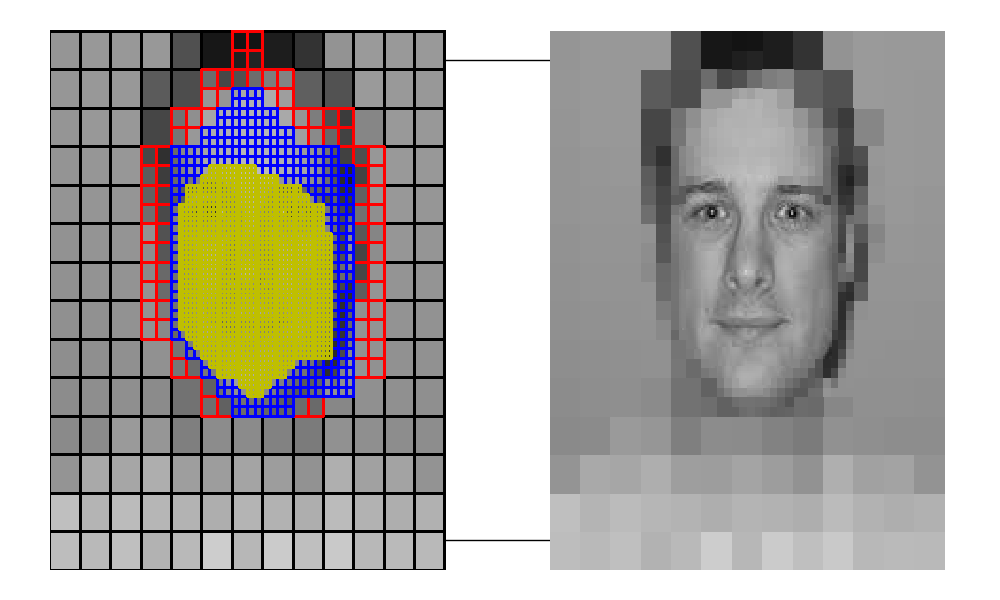
\includegraphics[bb=0bp 0bp 1000bp 600bp,clip,scale=0.45]{MDP_03}

\end{frame}

\begin{frame}{Adaptive Mesh Refinement (AMR)}


When this idea is followed through on structured meshes, it is often
called adaptive mesh refinement. Blocks are subdivided in areas of
refinement. Good for computer memory access, less good for physics.


\vspace{-2.65cm}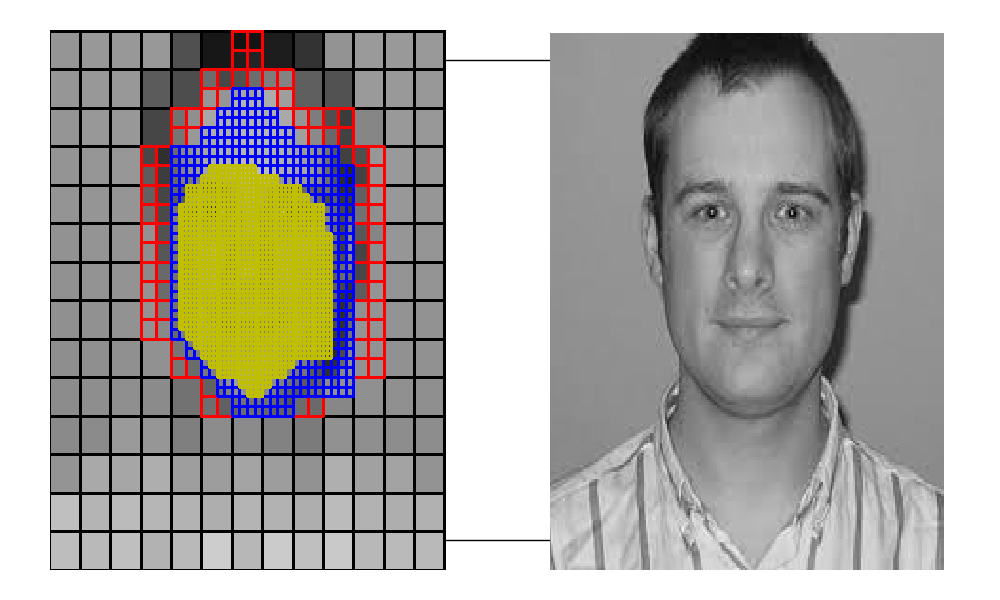
\includegraphics[bb=0bp 0bp 1000bp 600bp,clip,scale=0.45]{MDP_04}

\end{frame}



\section{Adaptive meshing for FEM}


\subsection{Forms of element adaptivity}
\begin{frame}{Finite elements: $h$ adaptivity}


\begin{center}
\vspace{-2cm}%
\begin{tabular}{ccc}
\multirow{3}{*}{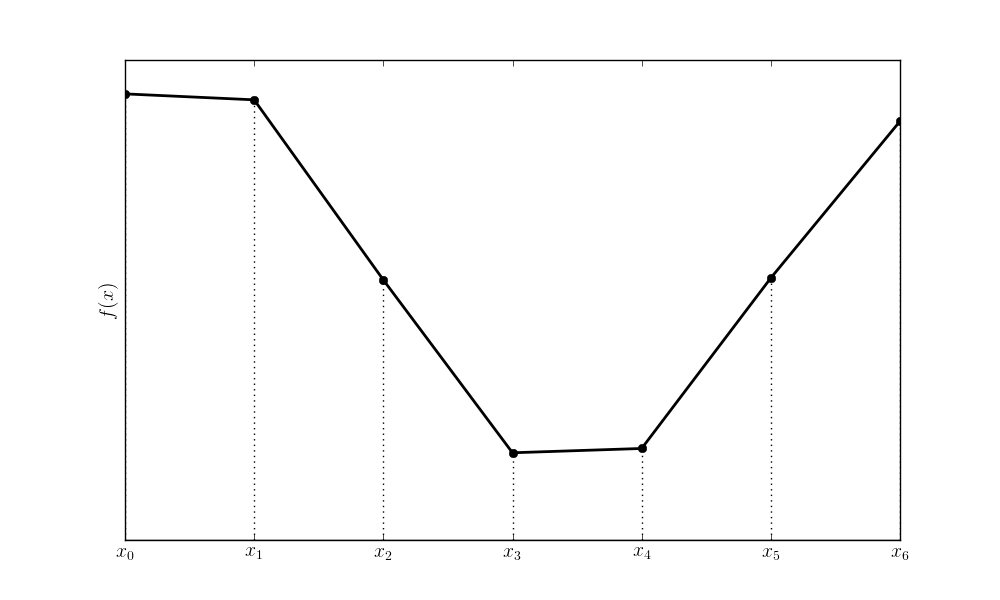
\includegraphics[width=0.4\textwidth]{adapt_0}} &  & \multirow{3}{*}{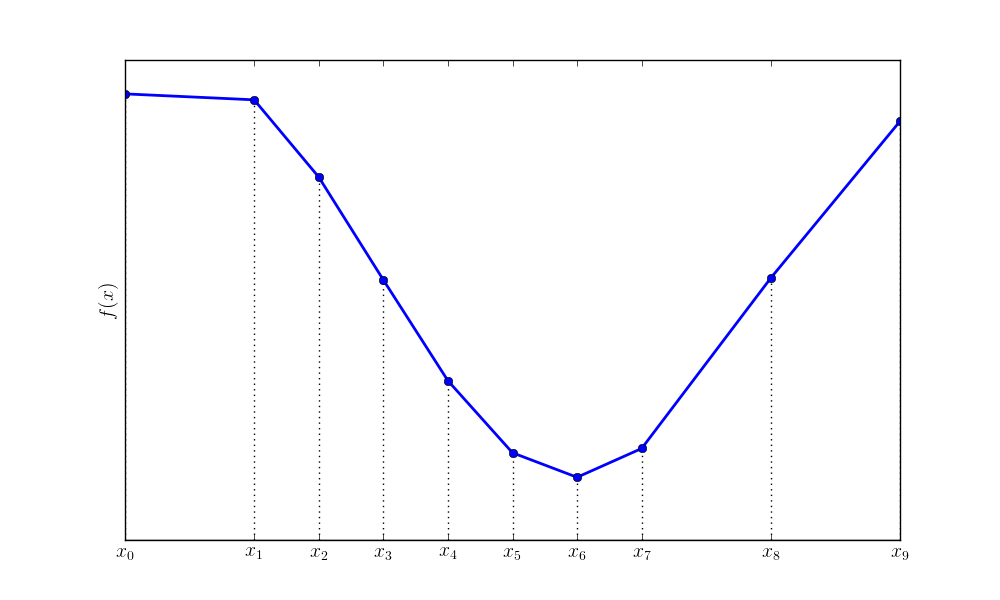
\includegraphics[width=0.4\textwidth]{adapt_h1}}\tabularnewline
 & $\Rightarrow$ & \tabularnewline
 & $h$ adapt & \tabularnewline
\end{tabular}
\par\end{center}


\vspace{1.cm}
\begin{itemize}
\item Adapt by using more, smaller elements ($h$ = step size)
\item Analagous to AMR.
\item Decreases error estimates, increases complexity (refinement)
\item Increases error estimates, decreases complexity (coarsening)
\item Implemented in Fluidity.
\end{itemize}
\end{frame}

\begin{frame}{Finite elements: $r$ adaptivity}


\begin{center}
\vspace{-2cm}%
\begin{tabular}{ccc}
\multirow{3}{*}{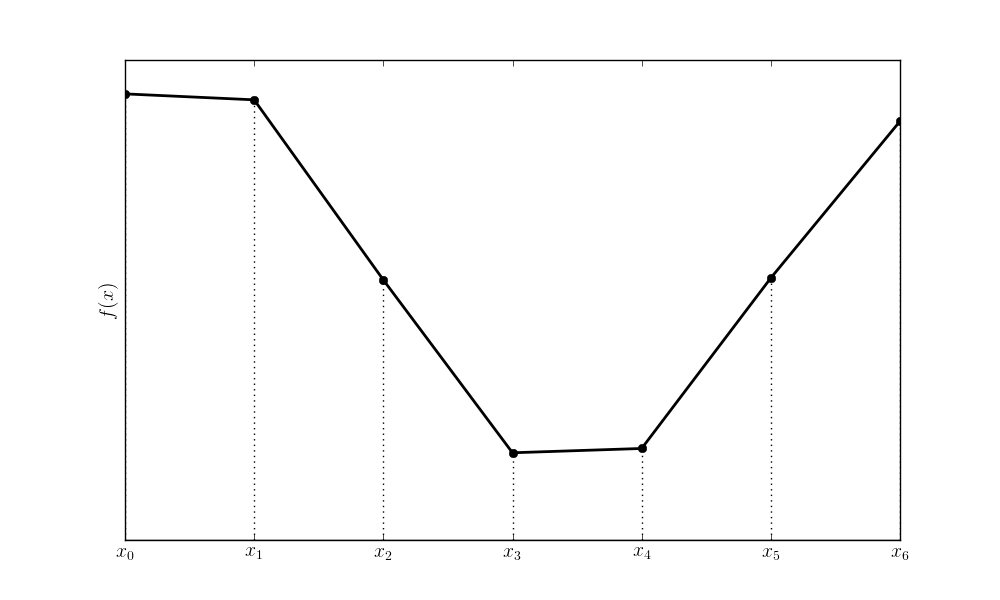
\includegraphics[width=0.4\textwidth]{adapt_0}} &  & \multirow{3}{*}{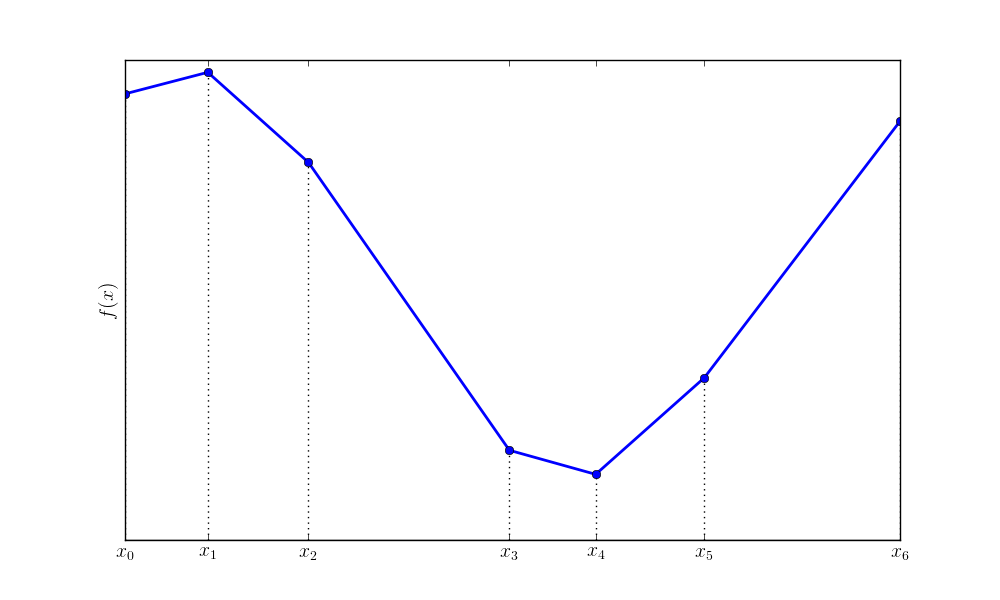
\includegraphics[width=0.4\textwidth]{adapt_r1}}\tabularnewline
 & $\Rightarrow$ & \tabularnewline
 & $r$ adapt & \tabularnewline
\end{tabular}
\par\end{center}


\vspace{1.cm}
\begin{itemize}
\item Adapt by repositioning nodes so that elements are ``better'' shape
\item Decreases error, maintains complexity.
\item Implemented in Fluidity.
\end{itemize}
\end{frame}

\begin{frame}{Finite elements: $p$ adaptivity}


\begin{center}
\vspace{-1cm}%
\begin{tabular}{ccc}
\multirow{3}{*}{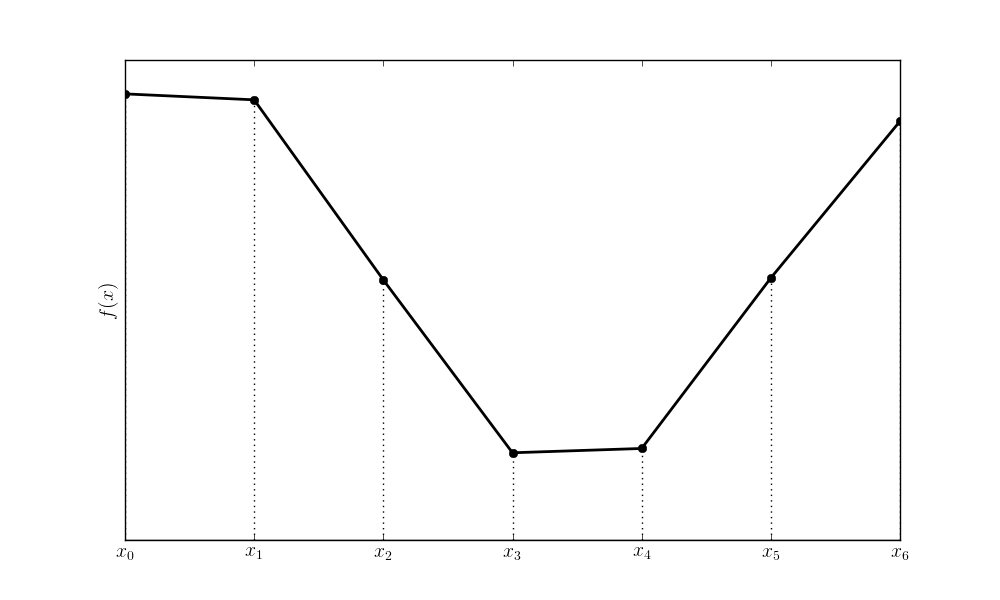
\includegraphics[width=0.4\textwidth]{adapt_0}} &  & \multirow{3}{*}{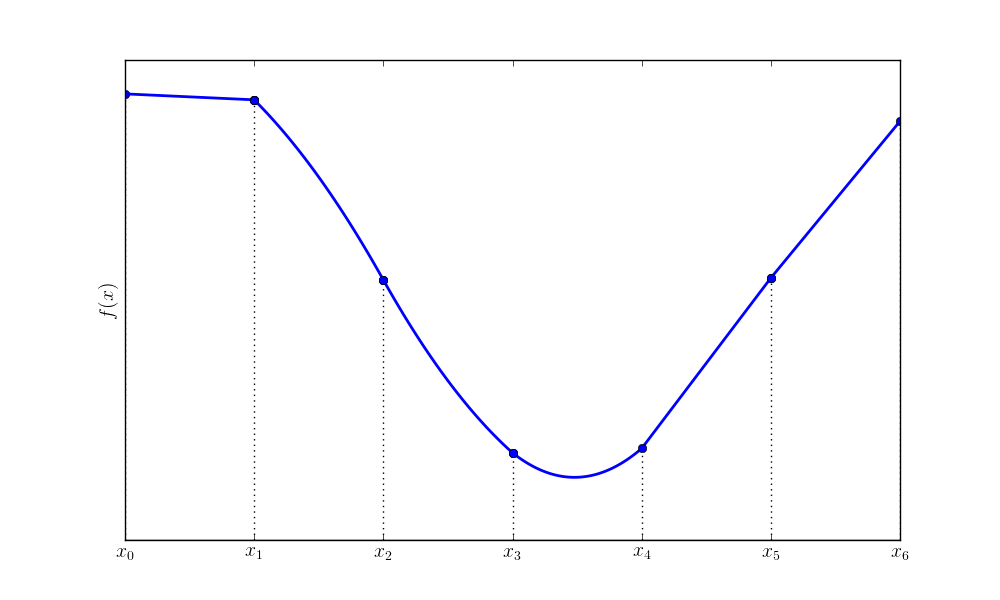
\includegraphics[width=0.4\textwidth]{adapt_p1}}\tabularnewline
 & $\Rightarrow$ & \tabularnewline
 & $p$ adapt & \tabularnewline
\end{tabular}
\par\end{center}


\vspace{1.cm}
\begin{itemize}
\item Adapt by using higher/lower order elements as required in different
parts of mesh
\item Decreases error estimates, increases complexity (refinement)
\item Increases error estimates, decreases complexity (coarsening)
\item Complex coupling with $h$ adaptivity.
\item Not currently implemented in Fluidity
\end{itemize}
\end{frame}



\subsection{Solution error and mesh resolution in FEM}
\begin{frame}{Revision of C�a's lemma}


C�a's lemma provides inequality.
\[
\mbox{error}:=\left\Vert \psi-\psi^{\delta}\right\Vert \leq\frac{\alpha C}{c}\sup_{\Omega_{i}}h_{i}\sup_{x\in\Omega}\left|\frac{\partial^{2}\psi}{\partial x^{2}}\right|
\]
Used this to show convergence as $h\rightarrow$0. But also a connection
to adaptive meshing. Go element by element
\[
\left\Vert \psi-\psi^{\delta}\right\Vert \leq\frac{\alpha}{c}\sum_{i}h_{i}^{2}\sup_{x\in\Omega_{i}}\left|\frac{\partial^{2}\psi}{\partial x^{2}}\right|.
\]



One definition of ``good'' mesh will minimise this representation
\emph{error estimate}. When $\left|\frac{\partial^{2}\psi}{\partial x^{2}}\right|$
is \emph{small}, element size $h_{i}$ can be \emph{large}, and
vice versa.

\end{frame}

\begin{frame}{Connection to mesh adaptivity}


\begin{center}
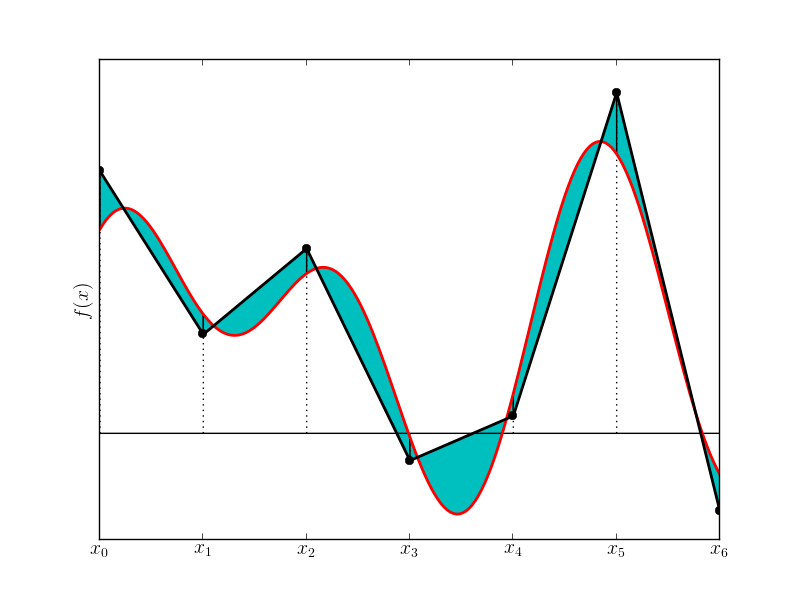
\includegraphics[height=0.9\textheight]{../IntroToFEM/adapt_ex1}
\par\end{center}

\end{frame}

\begin{frame}{Connection to mesh adaptivity}


\begin{center}
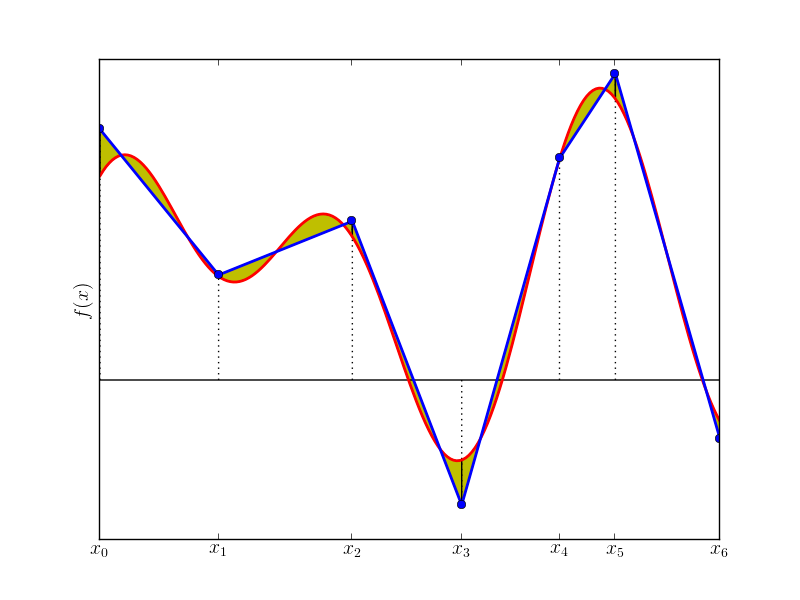
\includegraphics[height=0.9\textheight]{../IntroToFEM/adapt_ex2}
\par\end{center}


\end{frame}

\subsection{Mesh optimization}
\begin{frame}{Connection to mesh adaptivity}

\begin{block}{Problem: }


We don't know true solution,$\psi$, so can't find $\frac{\partial^{2}\psi}{\partial x^{2}}$
etc.

\end{block}


\begin{block}{Solution:}


We have an existing value of FE solution, $\psi^{\delta}$, Esimate
derivatives from that. 
\end{block}

In 2D/3D $\frac{\partial^{2}\psi}{\partial x^{2}}$ gets replaced
in the formula with the Hessian matrix,
\[
\mathcal{H}\left(\psi\right)=\left(\begin{array}{ccc}
\frac{\partial^{2}\psi}{\partial x^{2}} & \frac{\partial^{2}\psi}{\partial x\partial y} & \frac{\partial^{2}\psi}{\partial x\partial z}\\
\frac{\partial^{2}\psi}{\partial x\partial y} & \frac{\partial^{2}\psi}{\partial y^{2}} & \frac{\partial^{2}\psi}{\partial y\partial z}\\
\frac{\partial^{2}\psi}{\partial x\partial z} & \frac{\partial^{2}\psi}{\partial y\partial z} & \frac{\partial^{2}\psi}{\partial z^{2}}
\end{array}\right).
\]


\end{frame}

\begin{frame}{Mesh optimization}


Taking useful approximations to the error estimate, (see Chapter 7
of Fluidity manual) our goal for a mesh with ``nicely spread'' error
estimate is
\[
\frac{1}{\epsilon}\bm{v}_{k}^{T}\mathcal{M}\bm{v}_{k}=1
\]
where the $\bm{v}$s are the (vector) edges of the mesh, $\mathcal{M}=\mathcal{M}\left(\psi^{\delta}\right)$
is a function of the Hessian matrix (called the mesh metric tensor).
The \emph{interpolation error bound}, $\epsilon$, is a normalizing
factor which also nondimensionalizes the problem. 

\end{frame}

\begin{frame}{Notes on the interpolation error bound}


The $\epsilon$ has the same physical units as the field, $\psi$,
so can sensibly be specified in either:
\begin{enumerate}
\item absolute units (eg. 1 m/s for a velocity field) or,
\item relative units (eg. 5\% of the local value of $\psi^{\delta}$).
\end{enumerate}

It is also the principle control on the $\emph{number}$ of nodes
and elements required. It is thus often hard to guess without experimentation,
and simulation data from fixed resolution runs. In the absence of
other information, a fraction (e.g. 10\%) of the total variation in
$\psi$ expected across the entire domain may be a suitable first
choice.

\end{frame}

\begin{frame}{Examples of the Results}


\begin{center}
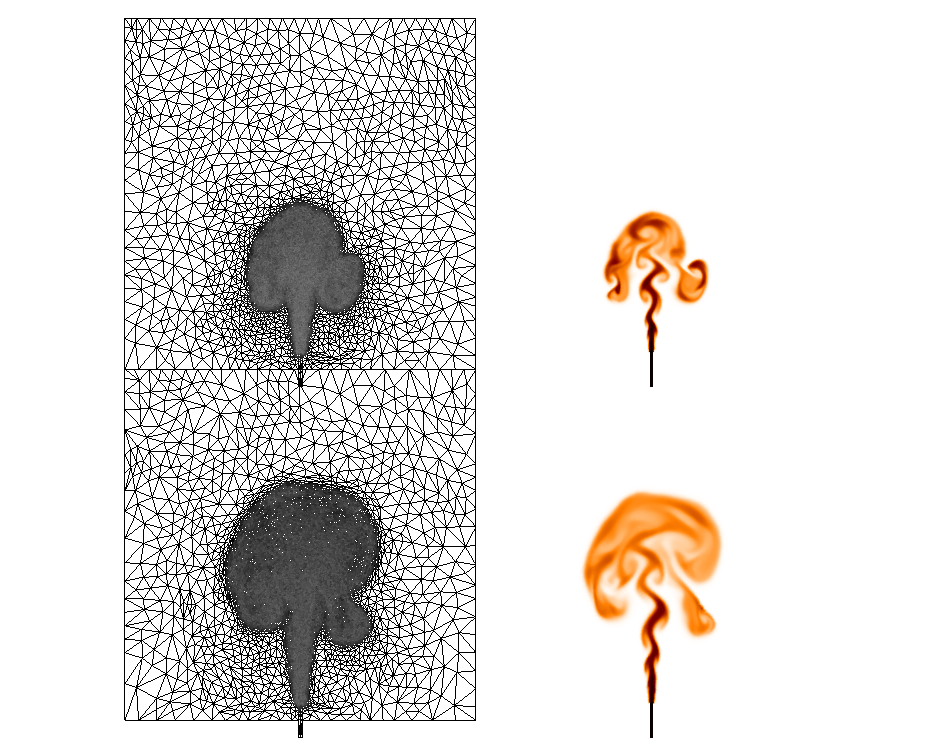
\includegraphics[height=0.9\textheight]{MeshAdaptivity}
\par\end{center}

\end{frame}

\begin{frame}{Points to remember}

\begin{itemize}
\item Mathematics has been given for a single variable, but in practice
CFD involves multiple prognostic variables.
\item Extension trivial, but each field requires own \emph{interpolation error bound}.
\item Haven't discussed the choice function in $\mathcal{M}$.
\item Implementation in parallel introduces additional complications
\item See Fluidity manual for more details.
\item Can minimize error estimate, but this may make numerics tricky. Answer
through additional constraints.
\end{itemize}
\end{frame}



\section{Further considerations}


\subsection{Bounds, gradation and metric advection}
\begin{frame}{Metric Tensor Bounds}


Usually desriable to have some additional constraints on the target
lengths in the mesh error metric tensor. Fluidity accepts 2 inputs,
giving the equation of bounding ellipses/ellipsoids on the edge lengths
in symmetric positive definite tensorial form:
\begin{columns}[c]


\column{5cm}


\begin{alignat*}{1}
\Phi & =\left(\begin{array}{cc}
a_{11} & a_{21}\\
a_{21} & a_{22}
\end{array}\right)\\
 & =R\left(\begin{array}{cc}
d_{1} & 0\\
0 & d_{2}
\end{array}\right)R^{T}
\end{alignat*}
$R=\left(\begin{array}{cc}
\cos\left(\theta\right) & -\sin\left(\theta\right)\\
\sin\left(\theta\right) & \cos\left(\theta\right)
\end{array}\right)$
\begin{alignat*}{1}
\left(\begin{array}{cc}
x & y\end{array}\right)\Phi^{-1}\Phi^{-1}\left(\begin{array}{c}
x\\
y
\end{array}\right) & =1.
\end{alignat*}




\column{5cm}


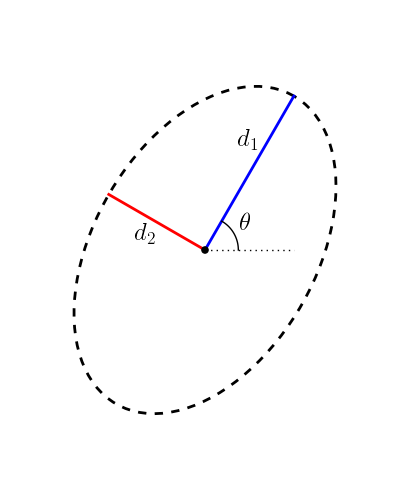
\includegraphics[width=0.9\columnwidth]{MetricEllipse}

\end{columns}

\end{frame}

\begin{frame}{Notes on Metric Tensor Bounds}

\begin{itemize}
\item Bounds are soft limits, not hard ones.
\item Interpolation error bounds should be primary control.
\item \emph{Maximum edge lengths} often come from the geometry.

\begin{itemize}
\item Also need to have enough resolution for phenomena to form.
\end{itemize}
\item \emph{Minimum edge lengths} often come from the physics.

\begin{itemize}
\item Also bad idea to have too many lengthscales in problem at once.
\end{itemize}
\item Example in domain with sides $L\times L\times H$
\[
\mbox{max.}=\left(\begin{array}{ccc}
\frac{L}{10} & 0 & 0\\
0 & \frac{L}{10} & 0\\
0 & 0 & \frac{H}{10}
\end{array}\right),\quad\mbox{min.}=\left(\begin{array}{ccc}
\frac{L}{100} & 0 & 0\\
0 & \frac{L}{100} & 0\\
0 & 0 & \frac{H}{100}
\end{array}\right)
\]

\end{itemize}
\end{frame}

\begin{frame}{Metric Advection}


The new mesh is optimized to have a small error metric at time it
is calculated. However, remeshing each time step would be both expensive
and potentially damaging to the solution. Ideally would like to have
bound on the error estimate which remains reasonable as the simulation
progresses. 


For advection dominated problems we can do this by treating the metric
tensor as ``just another variable''
\[
\frac{\partial\mathcal{M}}{\partial t}+\bm{u}\left(t_{0}\right)\cdot\nabla\mathcal{M}=0,\quad t\in[t_{0},t_{f}]
\]
And attempt to set
\[
\frac{1}{\epsilon}\max_{\tau\in[t_{0},t_{f}]}\left(\bm{v}_{k}^{T}\mathcal{M}\left(\tau\right)\bm{v}_{k}\right)=1.
\]


\end{frame}

\begin{frame}{Notes on Metric Advection}

\begin{itemize}
\item Metric advection increases limit on the period between adapts (usually)

\begin{itemize}
\item Rule of thumb for transient problem: 10 - 20 time steps.
\end{itemize}
\item Avoids issues with dissipation \& balance linked to frequent mesh
adaptation.
\item Fairly robust to choice of advection scheme, so long as it's stable

\begin{itemize}
\item (see next set of talks)
\end{itemize}
\item May increase problem sizes (larger areas with high resolution)
\item May misbehave if the physics of the system bifurcates.
\end{itemize}
\end{frame}

\begin{frame}{Metric Gradation}

\begin{itemize}
\item Often a bad idea to have length scales changing very rapidly between
neighbouring elements. (conditioning)
\item Post-processing of $\mathcal{M}$ can enforce smooth increases in
the metric away from minima:

\begin{itemize}
\item Isotropic $\|\bm{v}_{i}\|/\|\bm{v}_{j}\|\leq$\textrm{\textcolor{green}{1.5}}
if i, j are neighbouring edges (default)
\item anisotropic $\bm{v}_{i}\cdot\underline{\Gamma}\cdot\bm{v}_{j}\leq\|\bm{v}_{j}\|^{2}$
if i, j are neighbouring edges
\end{itemize}
\end{itemize}
\end{frame}

\begin{frame}{Notes on Metric Gradation}


A typical choice would be
\[
\underline{\Gamma}=\left(\begin{array}{cc}
1.5 & 0\\
0 & 1.5
\end{array}\right)\mbox{ or, to same result}\left(\begin{array}{cc}
1/1.5 & 0\\
0 & 1/1.5
\end{array}\right)
\]

\begin{itemize}
\item The default gradation is good unless there's a special reason to have
a very smooth variation.
\item Anisotropic gradation is more suited to anistropic problems (fronts/filaments/high
aspect ratios)
\item Sometimes want to limit individual element aspect ratios as well.
\end{itemize}
\end{frame}



\subsection{Variable mesh to mesh interpolation}
\begin{frame}{Mesh to Mesh interpolation}


Having found an improved mesh to represent our solutions, must still
transfer variable data (velocities, pressures etc) from the old mesh
onto the new one. This is the mesh to mesh interpolation problem.
Ideal method would:
\begin{itemize}
\item be fast computationally
\item be conservative where relevant
\item remain bounded (for data which have meaningful bounds)
\item return the original data for the original mesh
\end{itemize}
\end{frame}

\begin{frame}{Consistent Interpolation}


Conceptually simplest scheme is to set nodes of the new mesh to the
function values on the old mesh,
\[
\psi_{i}^{\mbox{new}}=\psi^{\mbox{new}}\left(\bm{p}_{i}\right)=\sum_{j}N_{j}^{\mbox{old}}\left(\bm{p}_{j}\right)\psi_{j}^{\mbox{old}}
\]



\begin{center}
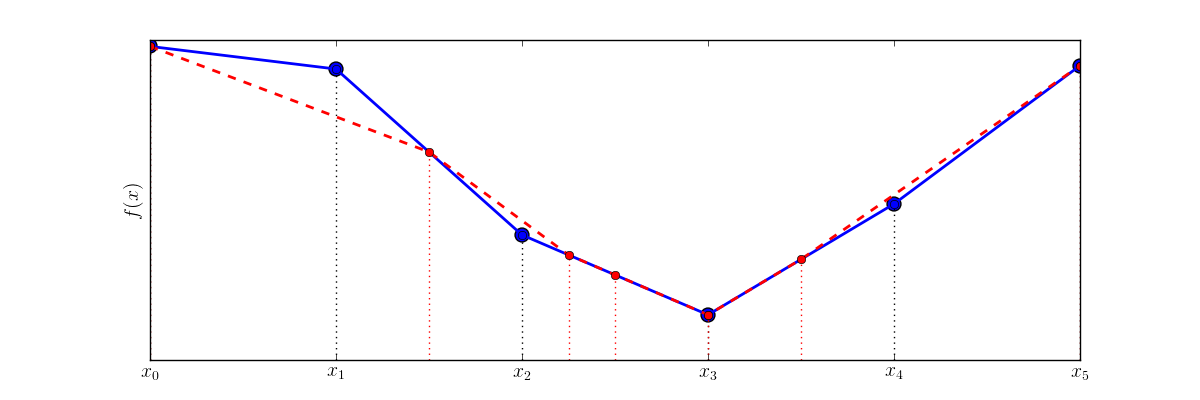
\includegraphics[width=1\textwidth]{ConsistentInterpolation}
\par\end{center}

\end{frame}

\begin{frame}{Notes on Consistent Interpolation}

\begin{itemize}
\item Fast.
\item Nonconservative.
\item Bounded.
\item Preserves data under identity mesh transformation.
\item Doesn't like discontinuous data.
\end{itemize}
\end{frame}

\begin{frame}{Galerkin projection}


A second option is to treat the problem
\[
\psi^{\mbox{new}}=\psi^{\mbox{old}}
\]
as a standard finite element problem. Obtain Galerkin projection equation
\[
\sum_{j}\int_{\Omega}N_{i}^{\mbox{new}}N_{j}^{\mbox{new}}\psi_{j}^{\mbox{new}}dV=\sum_{k}\int_{\Omega}N_{i}^{\mbox{new}}N_{k}^{\mbox{old}}\psi_{k}^{\mbox{old}}dV
\]



Left hand side is standard sparse mass matrix. The right hand side
is more complicated, but can be dealt with by supermeshing. 

\end{frame}

\begin{frame}{Notes on Galerkin projection}

\begin{itemize}
\item Significantly slower than consistent interpolation.
\item Conservative.
\item Not bounded (especially near discontinuities/extrema)
\item Preserves data under identity mesh transformation.
\end{itemize}
\end{frame}

\begin{frame}{Summary}

\begin{itemize}
\item Fluidity mesh adaptivity places resolution in regions of high curvature
\item Minimizes the interpolation error estimate for a given number of nodes
\item Uses $hr$ adaptive scheme.
\item Interpolate data from old to new mesh using chosen scheme.
\item For a new problem, usually best to do fixed resolution runs first.
\end{itemize}
\end{frame}

\begin{frame}{References}




\beamertemplatebookbibitems
\begin{thebibliography}{References}
\bibitem{key-2}Fluidity Manual\newblock AMCG\newblock 2014\beamertemplatearticlebibitems

\bibitem{key-1}C. C. Pain, A. P. Umpleby, et al. Tetrahedral mesh
optimisation and adaptivity for steady-state and transient finite
element calculations.\textit{\textcolor{green}{{} }}\textit{\textcolor{black}{Computer
Methods in Applied Mechanics and Engineering}}, 2001. 

\bibitem[Farrell]{key-4}P. E. Farrell and J. R. Maddison. Conservative
interpolation between volume meshes by local Galerkin projection.
\textit{\textcolor{black}{Computer Methods in Applied Mechanics and
Engineering}}, 2011.

\end{thebibliography}
\end{frame}

\end{document}
